\section{Statistics}

\subsection{Causal Inference}

La inferencia causal es el proceso de determinar el \textbf{efecto independiente de una variable} en un sistema más complejo. En general, este proceso es necesario cuando buscamos obtener conclusiones de datos pasados y en los que no es posible realizar un \textit{A/B testing}.

Existen 3 desafíos al realizar este proceso: 
\begin{itemize}
    \item \textbf{Cofounders}: Son aquellas variables que tienen un impacto en el \textit{outcome} y que incluso podrían tener un impacto en otras variables. 
    \item \textbf{Selection Bias}: Selección no representativa del grupo de control y tratamiento.
    \item \textbf{Counterfactuals}: Imputar valores en el grupo de control y tratamiento en base a \textit{Machine Learning} o algoritmos de \textit{Matching}. 
\end{itemize}

\begin{figure}[H]
    \center
    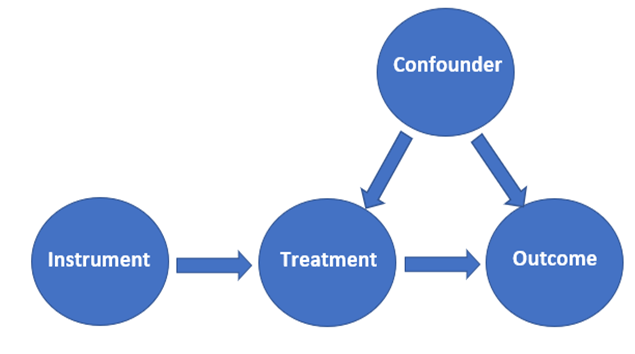
\includegraphics[scale=0.3]{notebooks/STATS/img/causal_inference_diagram.png}
    \caption{Casual Inference - DAG Diagram}
\end{figure}

Para resolver este problema, es necesario tomar algunos supuestos: 
\begin{enumerate}
    \item \textbf{Causal Markov Condition}: La influencia de las variables y el \textit{outcome} puede ser representado a través de un \textbf{Grafo Acíclico Dirigido (DAG)} en el que se asume la \textbf{condición de Markov}, es decir si $Y \rightarrow S \rightarrow C$, podemos asumir que $C \indep Y | S$
    \item \textbf{SUTVA}: (Stable Unit Treatment Value Assumption) El grupo de control y tratamiento \textbf{no tiene influencia el uno con el otro}. 
    \item \textbf{Ignorability}: Se excluye el ruido proveniente de cualquier otra fuente. 
\end{enumerate}

Consideremos el siguiente ejemplo en el que buscamos determinar si el efecto de un tratamiento tiene un impacto en una variable \textit{target}. 

\begin{figure}[H]
    \center
    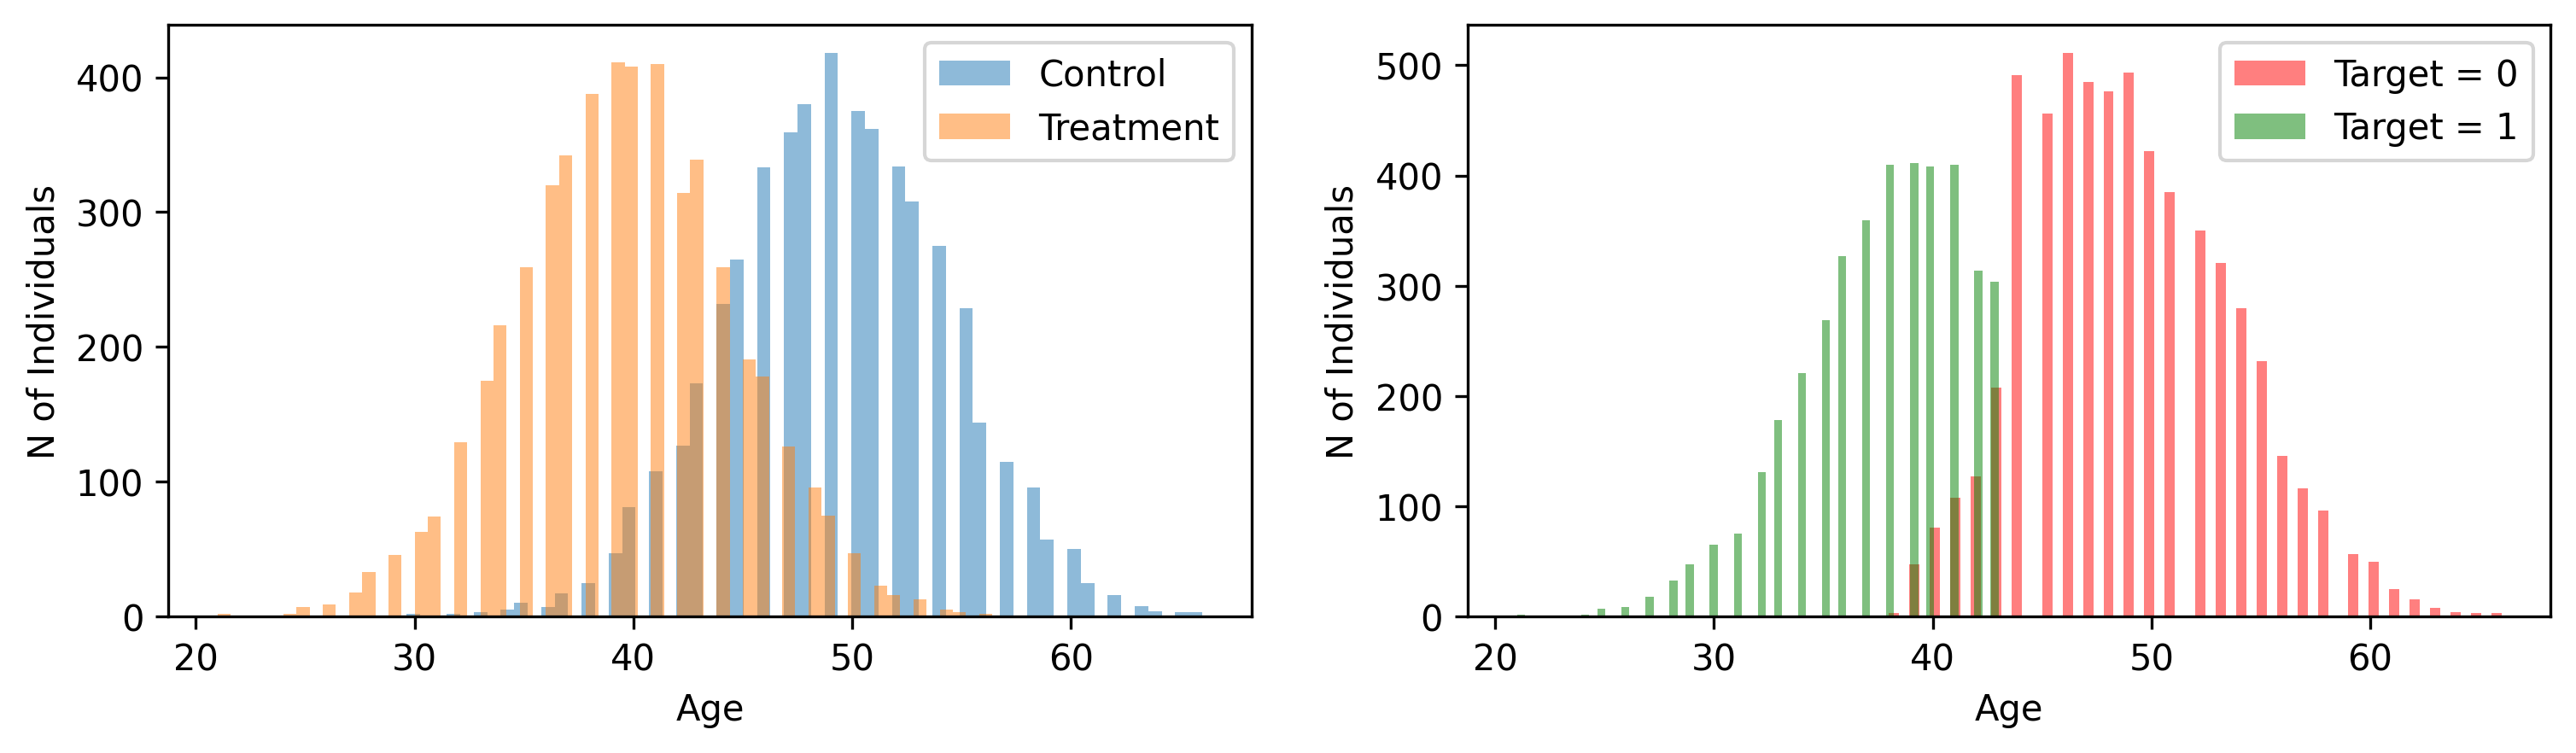
\includegraphics[scale=0.4]{notebooks/STATS/img/causal_inference_age_distribution.png}
    \caption{Casual Inference - Age Distribution}
\end{figure}

Vemos que existe un \textit{selection bias} pues el grupo de tratamiento y control pues tienen distribuciones de edad distintas. Existen múltiples enfoques para resolver este problema. 

\subsubsection{Matching Imputation}

Es posible utilizar un algoritmo de \textit{Matching} como \textit{NearestNeighbors} para imputar el posible \textit{outcome} que hubiese tenido un individuo al recibir o no el tratamiento. En nuestro ejemplo, para cada edad de los individuos del grupo de control, buscaríamos al sujeto con la edad más cercana en el grupo de tratamiento y imputaríamos su respuesta al tratamiento y viceversa. 

La efectividad del tratamiento se puede medir a través del promedio de los \textit{outcome} cuando reciben y cuando no reciben el tratamiento. 

\subsubsection{Two ML Models}

Este enfoque plantea entrenar 2 clasificadores, uno para el grupo de control y otro para el grupo de tratamiento. Sea $y_i$ el \textit{target}, $w$ si recibió el tratamiento y $X_i$ el conjunto de variables del modelo. Con esto, los output quedan definidos según $p(y_i = 1 | w = 1, X_i)$ y $p(y_i = 1 | w = 0, X_i)$. 
Definimos el valor ITE (\textit{Individual Treatment Effect}) según 
$$
\text{ITE} = \left [ p(y_i = 1 | w_i = 1, X_i) - p(y_i = 1 | w_i = 0, X_i) \right ]
$$
Así, si el valor de ITE es alto, implica que en el individuo $i$ el tratamiento $w$ \textbf{si tiene un efecto}. 

Hay que tener en consideración que este modelo requiere una \textbf{calibración} para asegurar que el \textit{output} de los modelos sean probabilidades.







